\documentclass[thesis,letterpaper,12pt]{utthesis}
\usepackage{graphicx}
\usepackage{biblatex}
\usepackage{algorithm}
\usepackage{algpseudocode}
\usepackage{booktabs}
\usepackage{tabularx}
\usepackage{array}
\usepackage{appendix}
\usepackage[T1]{fontenc}
\usepackage{amsmath}

\newcolumntype{Y}{>{\raggedright\arraybackslash}X}

\title{MENTOR-RL Methods}
\author{Peter Kruse}
\date{June 2026}

\addbibresource{references.bib}

\begin{document}
\maketitle

\section{Introduction and Motivation}

\subsection{Biological Interpretation as Mechanistic Discovery}
Biological interpretation involves the development and discovery of mechanistic relationships between biological entities such as genes, proteins, RNA, and other molecular components. Systems biology approaches this by studying the interactions between molecular entities rather than their individual properties~\cite{hartwell1999molecular, barabasi2004network}, seeking to identify \textit{modules}, groups of functionally related entities, and to characterize the mechanisms underlying their behavior. Because these interactions span multiple scales and regulatory layers, modern analysis relies on multiplex and multilayer representations that hold the same genes across several types of edge~\cite{barabasi2011network, ideker2012differential, mucha2010community, de2013mathematical}, over which propagation methods such as random walk with restart (RWR) identify functionally related neighborhoods~\cite{kohler2008walking, cowen2017network}. Module-level analysis has become foundational for identifying disease mechanisms, prioritizing drug targets, and interpreting polygenic phenotypes~\cite{menche2015uncovering}. Machine learning and artificial intelligence techniques such as iterative random forest (iRF)~\cite{basu2018iterative, cliff2019high} have accelerated this work by constructing biologically informed networks that scientists explore to generate mechanistic and functional hypotheses.

As these methods increase the resolution and scope of networks, biological interpretation has become increasingly mediated by large, multi-scale graph structures. To comprehensively examine these large biological networks and supporting databases, mechanistic exploration requires iterative querying and multi-step reasoning. Recent agentic interpretation systems such as eubiota~\cite{eubiota} and \textsc{Mentor-IA}~\cite{mentor-ia} demonstrate that provenance-preserving retrieval and tool-mediated synthesis can yield high-fidelity mechanistic narratives. However, these pipelines depend on frontier model inference and are not fully optimized as a trainable policy.

\subsection{Biological Interpretation is Bottlenecked by Human Cognition and Frontier Model Cost}
Although ML/AI methods such as \textsc{Mentor}~\cite{mentor} have refined mechanistic focus into groups of functionally related modules of genes, these modules can still be massive and intractable for individual researchers to systematically explore. Additionally, most research emphasizes a deep-but-narrow focus on a small subset of functionally related genes, which can overlook broader, yet biologically meaningful, network context, particularly in highly interactive systems such as living organisms. As biological networks grow in complexity, the combinatorial space of possible multi-hop interactions expands rapidly, while human interpretive capacity remains fixed.

While large language models (LLMs) can synthesize large volumes of information, frontier inference cost scales with exploration length and reasoning depth, limiting agentic deployment for long-horizon network traversal. This mismatch creates a scaling limit in biological mechanistic interpretation: rich relational structures can be computed, but downstream synthesis remains constrained by human bandwidth and model cost. Consequently, the speed, breadth, and contextual depth of mechanistic discovery are limited, particularly for complex traits, polygenic diseases, and multi-layer regulatory systems.

\subsection{AI-Guided Reasoning to Extend Mechanistic Interpretation Beyond Human Scale}
Open-source LLMs present an opportunity to aid scientists in mechanistic discovery tasks without being cost prohibitive. Language models reason more reliably when prompted to produce intermediate steps~\cite{wei2022chain, kojima2022large}, and equipping them with external tools supplies a layer of deterministic verification that reduces hallucination and preserves provenance~\cite{schick2023toolformer, yao2022react}. Adding an explicit verification stage improves factual reliability further, whether through iterative self-critique without weight updates~\cite{madaan2023selfrefine, shinn2023reflexion} or through a dedicated verifier with separate weights~\cite{eubiota}. Applied to gene set interpretation, this progression runs from precomputed language-model embeddings~\cite{chen2025simple}, through multi-step pipelines with database-backed self-verification~\cite{wang2025geneagent}, to multi-agent mechanistic synthesis~\cite{mentor-ia, eubiota}. None of these systems is trained end-to-end as a policy over verifiable rewards.

Reinforcement learning supplies the machinery to close that gap. Preference optimization aligns a policy to pairwise judgments, and direct preference optimization (DPO) does so without a separate learned reward model~\cite{christiano2017rlhf, ouyang2022instructgpt, dpo}. Policy gradient methods instead optimize against scalar rewards over complete rollouts~\cite{schulman2017proximal, shao2024deepseekmath}, and verifiable rewards have been shown to elicit long-horizon reasoning behavior at frontier scale~\cite{guo2025deepseek}. These methods have been applied to tool-using agents for browsing, large API vocabularies, and multi-step web tasks~\cite{nakano2021webgpt, qin2023toolllm, putta2024agent}, but not to a policy whose rewards are grounded in network-derived biological targets. We propose \textsc{Mentor-RL}, a model trained on biological ground truth and verifiable interaction objectives, enabling scalable mechanistic exploration without reliance on proprietary models. Leveraging open-source model offerings allows local deployment, with training costs amortized across many exploration sessions. Rather than replacing scientific judgment, \textsc{Mentor-RL} extends the interpretive bandwidth of researchers, enabling broader, faster, and more context-aware mechanistic discovery.

\subsection{A World Model of the Multiplex, Not a Graph Lookup Table}
Sequence models trained on synthetic tasks form internal, causal models of the process behind their data, and those models generalize to states never seen during training~\cite{li2023othello}. This works because the rules that generate the data are compact and recur across many examples, while the specific data does not. Two consequences shape this proposal. First, a model can learn the operators that regenerate structure, but it cannot memorize irreducible content that follows no compact rule, so biological edge weights, walk scores, and distances belong in the runtime rather than in the weights. Second, a world model emerges only under dense sampling of the generating process, which a single network queried with fixed templates cannot supply.

We therefore train \textsc{Mentor-RL} on a structured population of multiplex networks rather than on one. Every network in the population is built by the same rule: the predictive expression network (PEN) layers selected for a biological context define its gene universe, the remaining layers are induced on that universe, and the layers are stacked. Varying the context, whether a cell type, a tissue, a brain region, or an organ system, varies the resulting network while holding the construction rule fixed. We call this population the \textit{multiplex lattice}, and it supplies the dense sampling that a single network cannot.

The invariant we train on is therefore not any particular network or hierarchy, but the operator that maps a multiplex to its structure and the way layer composition drives that operator. We expect hierarchies to differ strongly across contexts, with distinct clades emerging in different cell types and regions. That divergence is the biology rather than an artifact: a model that has learned the operator will produce correspondingly different hierarchies for different contexts, and recovering the divergence correctly is a stronger result than reproducing conservation.

A hierarchy alone cannot serve as the world model, because it is a lossy abstraction of the multiplex it summarizes. Two clades that sit far apart in a tree may still be joined by short, biologically supported paths through bridge nodes in the underlying network, which is why a signal such as drug-target enrichment can appear in several distant branches and yet act through a single connected system. The model must hold the network itself and reason about the cross-clade connectivity that the tree suppresses. The hierarchy is the index used to find and prioritize; the network is where hypotheses are confirmed.

This proposal pursues four objectives. We define the multiplex lattice and ground it in a standard biological ontology, so that every network carries a canonical address and network composition is the join operation over that ontology. We design a supervised curriculum that teaches multiplex operators rather than graph content, holding the three structural views as co-equal targets and admitting a training example only when its target passes a typed validator against deterministic runtime output. We hand the resulting checkpoint to a tool-using agent, formalized as a sequential decision process over a structured state and scored by deterministic, schema-grounded rewards rather than proprietary judges. Finally, we make the world-model claim falsifiable through two flagship evaluations, generating a hierarchy for a context never seen in training and projecting a drug target onto the hierarchy before returning to the network to recover the connectivity that justifies it, supported by activation probes that test whether the recovered structure is causal rather than decorative.

\section{Proposed Methodology}\label{sec:methods}
Our methodology has four parts. Sections~\ref{sec:lattice} through~\ref{sec:pillars} define the training substrate: the lattice of multiplex networks, the ontology that addresses it, and the three structural views the model is required to hold. Sections~\ref{sec:graph-runtime} and~\ref{sec:sft-curriculum} describe the deterministic runtime and the supervised curriculum that builds the world model, and Section~\ref{sec:splits} defines the split and leakage protocol. Sections~\ref{sec:agent_loop} through~\ref{sec:rewards} formalize the mechanistic agent that the foundation checkpoint hands off to, together with its task corpora, trajectory generation, and reward functions. Section~\ref{sec:training} defines the staged training pipeline and curriculum, and Section~\ref{sec:eval} describes evaluation and benchmarking.

\subsection{The Multiplex Lattice}\label{sec:lattice}
Every multiplex in the lattice is built by one rule. The PEN layers selected for a context define its gene universe; HumanNet and the other non-PEN layers are induced on that universe, restricted to those genes and the edges among them; and all layers are then stacked into a multiplex. The backbone is therefore not shared across the lattice. It is an induced subgraph whose nodes and edges both follow from the PEN selection, so two contexts differ in their expression layers and in their induced backbone together.

The family this rule generates is nested and compositional. The finest grain is a single cell type, in one tissue, in one region. Combining cell types gives a tissue-level multiplex within a region, combining tissues gives a region-level multiplex, and combining regions builds up to the whole-brain multiplex we already hold. The same construction extends to other organ systems and to multiplexes that join organ systems, up to a whole-body multiplex. Disease-relevant networks, including the anxiety, suicide, pan-substance-use-disorder, and cardiac projections, are points in this same lattice rather than separate resources, which is what makes transfer between them meaningful.

Composition applies the same rule to a union. The gene universe of a combined multiplex is the union of its parts' PEN gene sets, the non-PEN layers are re-induced on that union, and the PEN layers are stacked. This has a direct consequence for training: a change of context is compound. Adding or removing a single PEN layer changes the gene universe and re-induces the backbone along with it, so a minimal pair of multiplexes differs by that layer together with its induced backbone, and the isolated single-layer effect is recovered only under a controlled ablation.

Before the full build, a divergence validation study confirms that different PEN selections do in fact produce divergent multiplexes, hierarchies, and connectivity, by comparing RWR-LOE neighborhoods, \textsc{Mentor}-derived hierarchies, and cross-clade connectivity across a first set of contexts. Strong divergence is the expected and desired result, and it is a precondition for everything downstream: it is what establishes that the lattice samples a generating process rather than re-presenting a single network under different names. This study also fixes parameters that remain provisional until it completes, including the sampling rates across lattice tiers and how many contexts are worth building at each tier.

\subsection{Context Ontology and Lattice Addressing}\label{sec:ontology}
The lattice is represented as a grounded ontology, so that every multiplex has a canonical and interoperable address and the composition operator has a defined domain. We build on existing community ontologies rather than a bespoke scheme, which lets the lattice inherit versioning, cross-species bridges, and alignment to the public single-cell corpora that also serve as data sources.

Each context is placed on two axes, with an optional third. Anatomy and regions are grounded in UBERON~\cite{uberon}, extended by human brain atlas terms where finer regional detail is required than UBERON carries. Cell types are grounded in the Cell Ontology~\cite{cellontology}, extended by the Provisional Cell Ontology for the transcriptomic brain types the Cell Ontology does not yet hold~\cite{pcl}. Developmental stage, where it matters, is grounded in HsapDv. The linkage between the two axes comes from the ASCT+B tables of the Human Reference Atlas~\cite{asctb}, which tie anatomical structures to their resident cell types and are maintained across the whole body, and node annotation follows the CELLxGENE schema~\cite{cellxgene} so that contexts align with public single-cell corpora. Because the Human Reference Atlas is a whole-body construction, extending the lattice from brain to other organ systems populates more of the same ontologies rather than replacing the stack.

A context is a node addressed by an anatomy term, a cell-type term, and a developmental stage, and it carries the PEN layers that define its gene universe together with the taxonomy cluster identifier that produced them. The resulting structure is a partial order rather than a tree, because a cell type recurs across regions and a combination joins several parents: a single cell type in a region sits beneath both the all-cell-types node for that region and the same cell type across the parent structure. Composition is the join in that partial order. It moves anatomy up the part-of hierarchy and cell types up the transcriptomic taxonomy from subcluster to cluster to supercluster, and the joined node's gene universe is the union of its parts' PEN gene sets with the non-PEN layers re-induced on it, exactly as Section~\ref{sec:lattice} specifies. Each node stores both identities, the ontology term for interoperability and the cluster identifier for provenance, and both are version-pinned alongside the graph version and layer-list hash, with an explicit mapping from PEN-derived types to taxonomy identifiers that keeps node identity stable when a taxonomy is re-versioned.

The ontology is supplied to the model as context and serves as the domain of the composition operator; it is not content baked into the weights. The model reads a provided ontology and navigates it, so the brain ontology is context and the same navigation transfers when the lattice extends to other organ systems. Navigation is trained as a relational operator: returning a node's parents, children, and siblings, naming the join of two nodes as the multiplex their union defines, and reporting the ontology distance between two contexts. That distance also indexes evaluation, letting us ask how strongly sibling cell types diverge relative to how strongly a child diverges from its parent.

\subsection{Three Structural Views}\label{sec:pillars}
The model is trained to hold three views of a multiplex, weighted equally, because each captures structure the others suppress.

The bottom-up view is the gene-centric neighborhood produced by random walk with restart lines of evidence (RWR-LOE)~\cite{kainer2025rwrtoolkit}. Applied to a seed gene, RWR-LOE walks the entire multiplex, treating each layer as an independent line of evidence, and returns every other gene ranked by propagation proximity to that seed. Rather than imposing a fixed neighborhood size, a geometric elbow filter places the cutoff at the bend in the score-versus-rank curve, so retaining the seed together with all genes above the cutoff yields one adaptive, seed-centered module per gene in the network. Operators over this view include rank and score lookup, comparison of two genes within one ranked vector, closest-$k$ retrieval, elbow reasoning, set relations between neighborhoods, leave-one-out support, layer ablation, and seed essentiality.

The top-down view is the hierarchy produced by \textsc{Mentor} (Multiplex Embedding of Networks for Team-Based Omics Research)~\cite{mentor}, which computes RWR embeddings for every gene across the layers of a multiplex, converts those embeddings into pairwise distances, and applies hierarchical clustering to yield a genome-wide dendrogram whose leaves are genes and whose internal nodes represent successively coarser functional groups. Cutting the dendrogram at a given merge height selects a family of nested modules spanning the entire gene universe of the network, so granularity is controlled by the height of the cut. Operators over this view include clade membership, the lowest common ancestor of a gene pair, the subtree induced by a cut, parent, child, and sibling relations, and within-clade cohesion. Every one of these targets is defined inside a single tree and is therefore alignment-free: hierarchies are compared across contexts by value, and no two trees ever need to be aligned to each other. This is what makes divergence trainable rather than an obstacle. Cut height doubles as a difficulty control, running from coarse, well-separated clades to fine, easily confused ones.

The third view is the connectivity of the underlying network, which the hierarchy necessarily suppresses. Because a dendrogram is a summary of a multiplex, distance in the tree is not distance in the network: two clades on distant branches may be joined by short, layer-supported paths through a small number of bridge nodes. Operators over this view include cross-clade path recovery, connector and bridge node identification, decomposition of a path by its supporting layers, cohesion tested against a null distribution, and calibrated refusal of the inference that separation in the tree implies separation in the network. Training this view as a first-class target is what keeps the model from reading the dendrogram as the whole truth, and it carries the calibration rules that prevent claiming a direct interaction where only a cross-layer route exists.

The three views are exercised together in the projection operation of Section~\ref{sec:flagship-projection}, which seeds a neighborhood on the network, tests that neighborhood against the hierarchy, and then returns to the network to justify what the hierarchy reported.

\subsection{Agent Loop Formulation}\label{sec:agent_loop}
\subsubsection{Loop Formalization}
We model mechanistic graph exploration as a sequential decision process executed by a single policy model with an internal self-verification step. The loop begins when the user provides a query, $q$, and optional evidence $e^{\text{user}}$, which may include text context, seed genes, or a multiplex network. These inputs initialize the working interpretation $I_0$ and the structured state $S_0$.

For each decision point $t < T_{\max}$, the current decision context is
\[
D_t = (q, e^{\text{user}}, I_t, S_t).
\]

Given $D_t$, the agent emits an action consisting of a textual reasoning step $r_t$ and an optional tool action $a_t$. The reasoning step specifies the current subgoal or interpretation update, while the tool action specifies a runtime-executable call. If a tool action is emitted, it is executed by a deterministic runtime $\varepsilon$; otherwise, the observation is empty.

After the action is produced and any deterministic tool calls are executed, the same policy enters a verification mode. Conditioned on the query, user-provided evidence, the current interpretation, the current structured state, and the current reasoning/action outputs, the verifier updates the interpretation and structured state, yielding $(I_{t+1}, S_{t+1})$. It also emits a continuation decision,
\[
z_t \in \{\texttt{continue}, \texttt{revise}, \texttt{stop}\},
\]
which determines whether the current interpretation should be extended, revised, or terminated. The decision \texttt{revise} indicates that the next iteration proceeds by correcting the interpretation and structured state rather than simply extending them.

The process repeats until either $z_t = \texttt{stop}$ or the maximum decision budget $T_{\max}$ is reached. At termination, $I_T$ and $S_T$ are returned as outputs. $I_T$ provides a human-readable answer to the query with respect to the accumulated evidence, while $S_T$ stores the corresponding verifiable outputs for reward computation and provenance preservation.

We formalize one iteration of the agent loop as
\[
r_t, a_t \sim \pi_{\theta}^{\mathrm{act}}(\cdot \mid D_t), \qquad
o_t = \varepsilon(a_t), \qquad
I_{t+1}, S_{t+1}, z_t \sim \pi_{\theta}^{\mathrm{verify}}(\cdot \mid r_t, a_t, o_t, D_t),
\]
where $r_t$ is the agent's textual reasoning or subgoal, $a_t$ is the optional tool action, and $o_t$ is the observation returned by the deterministic runtime $\varepsilon$, with $\varepsilon(\varnothing)=\varnothing$ by convention. The policies $\pi_{\theta}^{\mathrm{act}}$ and $\pi_{\theta}^{\mathrm{verify}}$ denote two prompting modes of the same underlying model, sharing weights so that biological vocabulary and tool-use competence learned in one mode transfers to the other. We treat the risk that the verifier collapses as a monitoring concern during training, discussed in Section~\ref{sec:limitations}. At each decision point, the pair $(I_t, S_t)$ represents the current mechanistic hypothesis, with $I_t$ serving as a human-readable view and $S_t$ as a machine-readable view of the same underlying state. The full agent loop algorithm is detailed in Algorithm~\ref{alg:agent-loop}.

\begin{algorithm}[t]
\caption{The \textsc{Mentor-RL} agent loop}
\label{alg:agent-loop}
\begin{algorithmic}[1]
\Require query $q$, user evidence $e^{\text{user}}$, maximum decision budget $T_{\max}$, deterministic runtime $\varepsilon$
\State Initialize working interpretation $I_0$ and structured state $S_0$ from $(q, e^{\text{user}})$
\State $T \gets 0$
\For{$t = 0, 1, \dots, T_{\max}-1$}
    \State $D_t \gets (q, e^{\text{user}}, I_t, S_t)$
    \State $(r_t, a_t) \sim \pi_{\theta}^{\mathrm{act}}(\cdot \mid D_t)$
    \If{$a_t \neq \varnothing$}
        \State $o_t \gets \varepsilon(a_t)$
    \Else
        \State $o_t \gets \varnothing$
    \EndIf
    \State $(I_{t+1}, S_{t+1}, z_t) \sim \pi_{\theta}^{\mathrm{verify}}(\cdot \mid r_t, a_t, o_t, D_t)$
    \State $T \gets t+1$
    \If{$z_t = \texttt{stop}$}
        \State \textbf{break}
    \EndIf
\EndFor
\State \Return final interpretation $I_T$ and structured state $S_T$
\end{algorithmic}
\end{algorithm}

\begin{figure}[htb!]
    \centering
    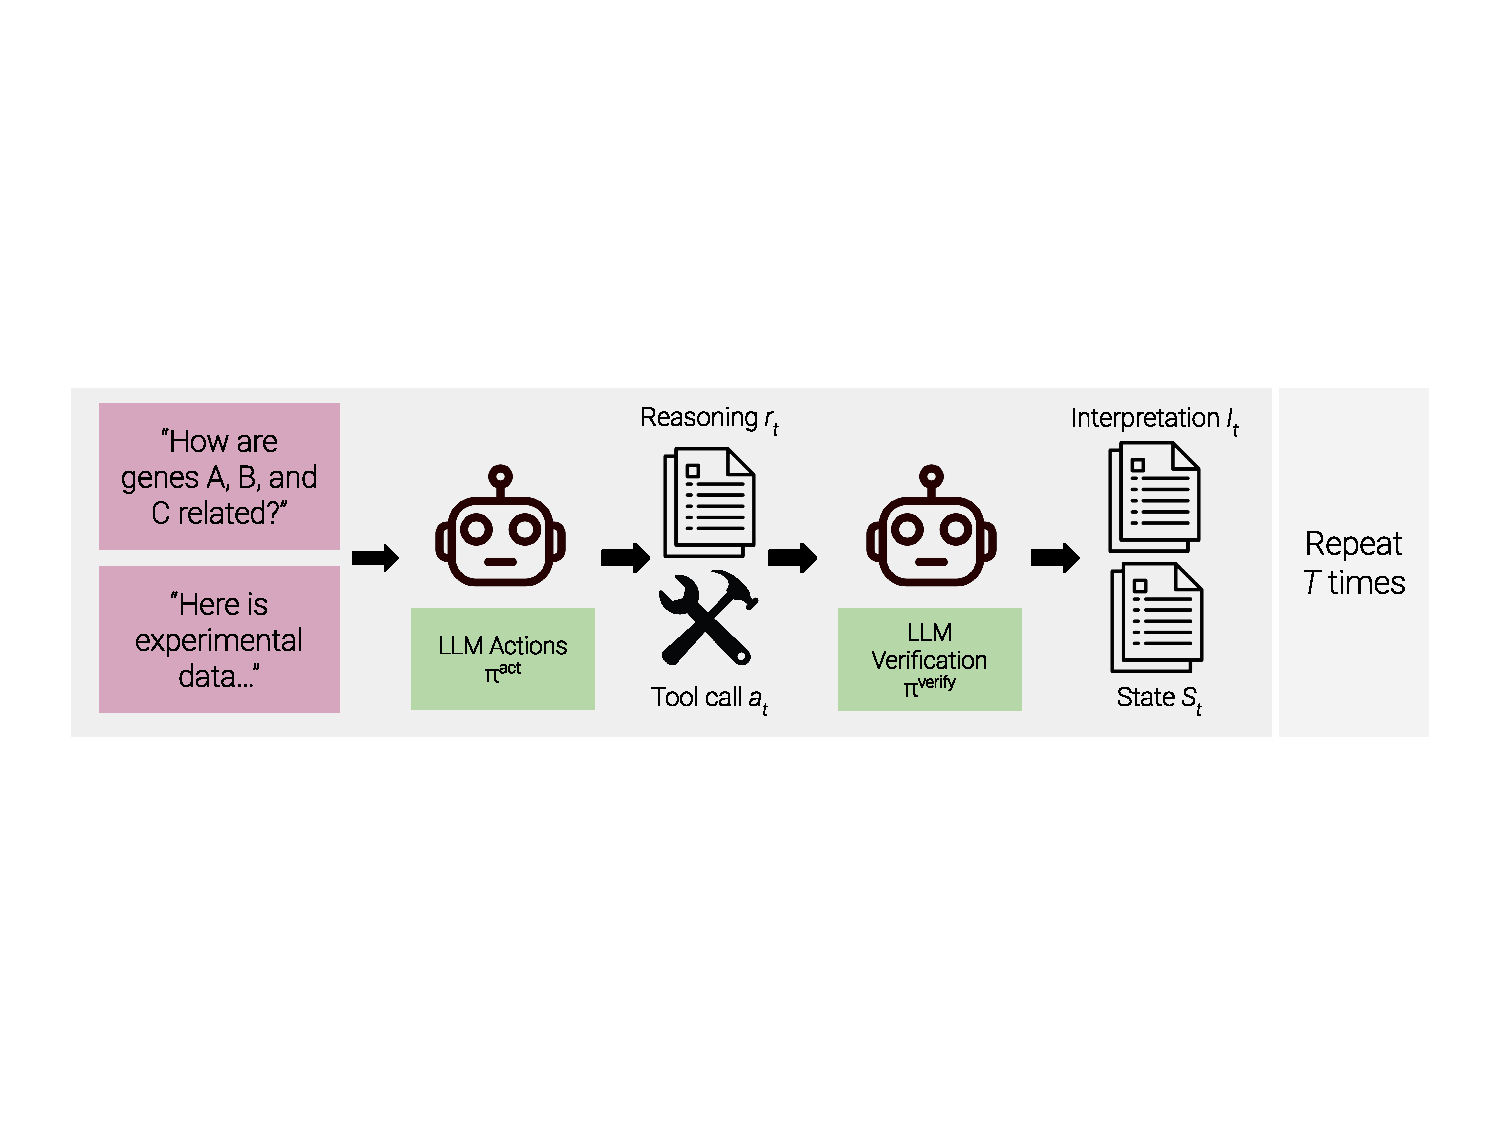
\includegraphics[width=\linewidth]{img/agent_loop.pdf}
    \caption{The \textsc{MENTOR-RL} agent loop.}
    \label{fig:agent-loop}
\end{figure}

\subsubsection{Working Interpretation}
The working interpretation $I_t$ is the human-readable form of the current mechanistic hypothesis and contains:
\begin{enumerate}
    \item the current mechanistic claim,
    \item the main evidence supporting that claim,
    \item any uncertainty, conflict, or alternative explanation,
    \item the next question or subgoal the model is trying to resolve.
\end{enumerate}

\subsubsection{Structured State}\label{sec:structured_state}
The structured state $S_t$ stores the same hypothesis in a machine-readable form suitable for tool execution, reward computation, and provenance tracking. It contains:
\begin{enumerate}
    \item the user-provided anchors $(q, e^{user})$,
    \item the current relationship status (unknown, partially observed group, validated group, multiple groups, or insufficient support) $(rel_t)$,
    \item the current predicted group or groups $(G_t)$,
    \item the evidence and provenance collected so far $(E_t)$,
    \item the current predicted mechanistic labels, each tied to the evidence handles that support it,
    \item the tool-use counters recording total and invalid tool calls $(n_{total}, n_{inv})$,
    \item the remaining budget and continuation state, and, at termination, the recorded termination signal $((T_{\max} - T), z_t)$.
\end{enumerate}

\subsection{Task Outputs and Mechanistic Targets}\label{sec:task}

\subsubsection{Final Interpretation}
The final outputs of the model are the terminal interpretation $I_T$ and the terminal structured state $S_T$. Together, these outputs must support four cases: completion of a partially observed mechanistic group, explanation of an already coherent group, refinement of a noisy group, and recognition that no single shared mechanism is supported. The final interpretation states which case is supported by the evidence, summarizes the main evidence for that claim, and links the evidence to the claim through reasoning traces and tool calls. It also records uncertainty or abstention when evidence is incomplete. If the loop terminates with $z_t = \texttt{stop}$, the next subgoal field is left blank. If the loop terminates because the decision budget $T_{\max}$ is exhausted, the interpretation may include a recommended next subgoal to guide further exploration.

\subsubsection{Final Structured State}
The final structured state is a schema-enforced JSON object. It contains the same components defined in Section~\ref{sec:structured_state}, but with finalized values for relationship status, predicted groups, collected evidence, and mechanistic labels. These values are used for reward evaluation and provenance tracking. The final structured state also records whether termination occurred because the model emitted $z_t = \texttt{stop}$ or because the budget $T_{\max}$ was exhausted. If the budget is exhausted, the remaining budget is $0$; if the model stops early, the remaining budget is $T_{\max} - T$.

\subsubsection{Supported Task Cases}
We support four output cases during training to reflect the variability of experimental evidence that users may provide:
\begin{enumerate}
    \item partial group completion,
    \item mechanism explanation for an already related group,
    \item group refinement from a noisy module,
    \item no single shared mechanism.
\end{enumerate}

Partial group completion occurs when the user provides a subset of related genes; the model expands this subset into a larger mechanistically related group and explains it. Mechanism explanation occurs when the user provides a complete module; the model explains the mechanism without unnecessary expansion. Group refinement occurs when the user provides a known module with several unrelated noise genes; the agent refines the group so that it contains only mechanistically related genes. Finally, in the no shared mechanism case, the user provides genes that do not support one coherent mechanism, and the model either splits them into multiple groups or returns insufficient support.

\subsubsection{Targets for Training and Evaluation}
We define two complementary target types for training and evaluation. \textbf{Module membership targets} are the hidden gene sets drawn from either \textsc{Mentor}-derived dendrogram modules or elbow-filtered RWR-LOE modules (Sections~\ref{sec:mentor-corpus} and~\ref{sec:loe-corpus}). These targets are only used for scoring: the agent never observes hidden module members and must recover them through exploration. These modules supply the supervised signal for set-level recovery, refinement, and abstention.

Because dendrogram modules are derived computationally from multiplex structure, they offer genome-wide coverage, but often without per-entry experimental annotations. \textbf{Mechanistic evidence targets} therefore score the quality of a final explanation against the evidence retrieved during exploration, such as enrichment, annotation, and graph support. This allows interpretations to be rewarded for being grounded in evidence rather than simply matching a pre-defined annotation, which encourages the exploration of novel biology beyond existing databases.

\subsection{Data, Resources, and Environment}\label{sec:data}
Our dataset is constructed from a combination of existing internal tool infrastructure, open-source biological resources, and graph exploration environments.

\subsubsection{Warm-Start SFT Dataset} 
We first construct a warm-start SFT subset from the \textsc{Mentor-IA} tool stack~\cite{mentor-ia}, including gene metadata, gene ontology (GO) annotations, pathway membership, and literature evidence. These data are retrieved via MyGene.info~\cite{mygene.info} and Europe PMC~\cite{europepmc}. This warm-start subset covers four task families:
\begin{enumerate}
    \item entity normalization, such as resolving gene names and synonyms to canonical identifiers,
    \item annotation retrieval, such as returning GO terms, localization, and pathway information for a gene or gene set,
    \item literature-grounded extraction, such as identifying relevant genes, pathways, or mechanisms from retrieved abstracts, and
    \item evidence-to-finding generation, which converts retrieved tool outputs into short, grounded mechanistic statements.
\end{enumerate}

We include tool-enabled (open-book) and tool-disabled (closed-book) questions, with open-book examples emphasized to promote schema-valid tool use and evidence grounding, and closed-book examples used to strengthen biological vocabulary and lightweight recall. To make this stage reproducible, API responses and database versions will be cached during dataset construction.

To make the warm-start SFT stage concrete, we define a core tool vocabulary derived from the existing \textsc{Mentor-IA} infrastructure~\cite{mentor-ia} in Table~\ref{tbl:tools}. Early SFT emphasizes schema-valid biological annotation and enrichment calls, while graph-exploration and RWR++ operators are introduced during DPO and online RL.

\begin{table}[p]
\centering
\caption{Tool vocabulary for the \textsc{Mentor-RL} agent. Related RWR++ calls are grouped by function while preserving the model-facing tool names.}
\label{tbl:tools}
\scriptsize
\setlength{\tabcolsep}{3pt}
\renewcommand{\arraystretch}{0.95}
\begin{tabularx}{\textwidth}{@{}>{\raggedright\arraybackslash}p{0.34\textwidth} >{\raggedright\arraybackslash}X >{\raggedright\arraybackslash}p{0.25\textwidth} >{\raggedright\arraybackslash}p{0.08\textwidth}@{}}
\toprule
\textbf{Tool(s)} & \textbf{Purpose} & \textbf{Primary inputs} & \textbf{Stage} \\
\midrule
\texttt{query\_mygene} & Gene metadata, GO terms, pathways, and summaries & \texttt{query}; requested \texttt{fields} & SFT \\
\midrule
\texttt{enrich\_gene\_set} & Functional enrichment over a candidate gene set & \texttt{genes}; \texttt{background}; \texttt{top\_k}; threshold & SFT, DPO, RL \\
\midrule
\texttt{get\_neighbors}; \texttt{induce\_subgraph} & Local native graph and induced-subgraph evidence & gene or gene-set identifiers; layers & DPO, RL \\
\midrule
\texttt{rwr}; \texttt{rwr\_loe}; \texttt{shortest\_paths} & RWR++ expansion, leave-one-out relatedness, and path evidence & seed, query, source, or target genes; layers; \texttt{top\_k} & DPO, RL \\
\midrule
\texttt{get\_rank}; \texttt{get\_distance}; \texttt{get\_spearman}; \texttt{get\_pearson}; \texttt{get\_dot\_similarity} & Rank, distance, and vector-similarity comparisons & paired genes; metric; layers & DPO, RL \\
\midrule
\texttt{get\_rank\_vector\_summary}; \texttt{get\_encoding\_summary} & Compact rank-vector and encoding summaries & seed or query genes; layers; \texttt{top\_k} & DPO, RL \\
\midrule
\texttt{get\_gene\_layers}; \texttt{get\_nodes\_by\_layer}; \texttt{get\_layer\_stats}; \texttt{get\_path\_layer\_counts}; \texttt{get\_component\_summary} & Layer membership, layer statistics, path support, and components & genes or layers, depending on query & DPO, RL \\
\midrule
\texttt{get\_seed\_essentiality}; \texttt{get\_layer\_ablation}; \texttt{get\_node\_perturbation} & Stability, ablation, and perturbation analyses & seed or perturbation genes; layers; \texttt{top\_k} & DPO, RL \\
\bottomrule
\end{tabularx}
\end{table}

\subsubsection{\textsc{Mentor}-Derived Training Corpus}\label{sec:mentor-corpus}
After constructing the warm-start SFT dataset, we create two complementary module corpora that together supply the hidden targets for trajectory generation: a \textsc{Mentor}-derived corpus (this section) and an RWR-LOE corpus (Section~\ref{sec:loe-corpus}). We first parse the genome-wide \textsc{Mentor} dendrogram into modules, where each module is the gene set of a dendrogram subtree. We partition the modules into train, validation, and test splits to prevent leakage across stages.

For each module $C_{\text{module}}$ of size $n$, we deterministically materialize up to four task instances, one per case in Section~\ref{sec:task}. This ensures that all four task types are represented for as many modules as possible rather than sampled independently. The \texttt{explanation} instance uses the full module as input, $C^{\text{in}} = C_{\text{module}}$. The \texttt{recovery} instance drops $k_{\text{drop}}$ genes from the module, $C^{\text{in}} = C_{\text{module}} \setminus G_{\text{drop}}$, and the \texttt{refinement} instance adds $k_{\text{add}}$ noise genes, $C^{\text{in}} = C_{\text{module}} \cup G_{\text{add}}$. In both the recovery and refinement cases, the hidden target remains $C = C_{\text{module}}$. The number of genes added or dropped scales with the task difficulty and module size, so that harder instances perturb a larger fraction of the module. The \texttt{none} instance constructs a pseudo-module of unrelated genes as input with hidden target $C = \varnothing$.

Noise and \texttt{none} genes are drawn from difficulty-modulated \textit{dendrogram distance bands}, which are defined by walking up the module's ancestry in the tree, so that difficulty controls how topologically close the distractors are to the module. Additionally, \texttt{none} genes are constrained to be conflict-free (i.e. they are not related to each other), so that sampled genes do not form a coherent module themselves. All selection is deterministic given a fixed seed, making the corpus reproducible. The resulting \textsc{Mentor}-based corpus provides supervision for schema-valid tool use and for the terminal outputs of Section~\ref{sec:task}.

\begin{algorithm}[t]
\caption{Creation of the \textsc{Mentor}-derived module training corpus}
\label{alg:mentor-module-corpus}
\begin{algorithmic}[1]
\Require dendrogram $D$, multiplex $M$, difficulty map $\delta$

% initialize modules from the dendro, parsing into train/val/test splits
\State Parse the genome-wide \textsc{Mentor} dendrogram $D$ over multiplex $M$ into modules $\{C_{\text{module}}\}$
\State Partition modules into train/validation/test splits at the module level

% loop through each module and create task instances for each case w/ set difficulty and size
\For{each module $C_{\text{module}}$ in split with difficulty map $\delta$}
    \State $n \gets |C_{\text{module}}|$

    \State \textbf{// explanation}
    \State emit $(C^{\text{in}} = C_{\text{module}},\; C = C_{\text{module}},\; \texttt{explanation},\; rel=\texttt{validated\_group})$

    \State \textbf{// recovery}
    \State $k_{\text{drop}} \gets \textsc{DropCount}(n, \delta_{\text{rec}})$;\quad $G_{\text{drop}} \gets \textsc{DetSelect}(C_{\text{module}}, k_{\text{drop}})$
    \State emit $(C^{\text{in}} = C_{\text{module}} \setminus G_{\text{drop}},\; C = C_{\text{module}},\; \texttt{recovery},\; rel=\texttt{validated\_group})$

    \State \textbf{// refinement}
    \State $k_{\text{add}} \gets \textsc{NoiseCount}(n, \delta_{\text{ref}})$;\quad $G_{\text{add}} \gets \textsc{DendroNeg}(C_{\text{module}}, k_{\text{add}}, \delta_{\text{ref}})$
    \State emit $(C^{\text{in}} = C_{\text{module}} \cup G_{\text{add}},\; C = C_{\text{module}},\; \texttt{refinement},\; rel=\texttt{validated\_group})$

    \State \textbf{// none}
    \State $G_{\text{none}} \gets \textsc{DendroNeg}(C_{\text{module}}, n, \delta_{\text{none}},\, \text{conflict\_free})$
    \State emit $(C^{\text{in}} = G_{\text{none}},\; C = \varnothing,\; \texttt{none},\; rel=\texttt{insufficient\_support})$
\EndFor
\State \Return all task instances
\end{algorithmic}
\end{algorithm}

\subsubsection{RWR-LOE Module Corpus}\label{sec:loe-corpus}
In addition to the top-down, hierarchical \textsc{Mentor}-derived module corpus, we create a corpus of RWR-LOE exploration across all genes in the multiplex to provide a bottom-up complement. For each gene $g$ in the same multiplex universe as the \textsc{Mentor} dendrogram, we run \texttt{rwr\_loe}$(g)$ to obtain a propagation score and rank for every other gene in the network. We then apply the RWR++ elbow filter to the score-versus-rank curve for that seed, yielding an adaptive cutoff rank $r^\star_g$. The LOE module is defined as $C^{\text{loe}}_g = \{g\} \cup \{v : \mathrm{rank}_g(v) \le r^\star_g\}$, producing a single seed-specific module per gene without imposing a fixed module size.

For each module, we materialize the same four task instances as the \textsc{Mentor}-derived corpus. For difficulty control, we substitute RWR-LOE rank bands for dendrogram distance bands: noise and \texttt{none} genes are drawn from ranks just beyond, moderately beyond, or far beyond the seed's elbow cutoff. We partition RWR-LOE modules into train, validation, and test splits independently of the \textsc{Mentor}-derived modules, and module-size bins are assigned after construction from the realized values of $|C^{\text{loe}}_g|$. The two corpora are complementary: \textsc{Mentor} modules capture top-down, hierarchical functional organization, while RWR-LOE modules reflect bottom-up, seed-centered topology.
\begin{algorithm}[t]
\caption{Creation of the RWR-LOE module training corpus}
\label{alg:loe-module-corpus}
\begin{algorithmic}[1]
\Require multiplex $M$, gene universe $\mathcal{G}$, elbow-filter parameters $\phi$, difficulty map $\delta$
\State Partition $\mathcal{G}$ into train/validation/test splits at the gene level
\For{each gene $g \in \mathcal{G}$}
    \State Run $\texttt{rwr\_loe}(g, M)$ to obtain scores $s_g$ and ranked list $L_g$
    \State $r^\star_g \gets \textsc{ElbowCutoff}(L_g, s_g, \phi)$
    \State $E_g \gets \{v \in L_g : \mathrm{rank}_g(v) \le r^\star_g\}$
    \State $C^{\text{loe}}_g \gets \{g\} \cup E_g$,
           \quad $n \gets |C^{\text{loe}}_g|$
    \State \textbf{// explanation}
    \State emit $(C^{\text{in}} = C^{\text{loe}}_g,\; C = C^{\text{loe}}_g,\;
           \texttt{explanation},\; rel=\texttt{validated\_group})$

    \State \textbf{// recovery}
    \State $k_{\text{drop}} \gets \textsc{DropCount}(n, \delta_{\text{rec}})$;
           \quad $G_{\text{drop}} \gets \textsc{DetSelect}(C^{\text{loe}}_g,
           k_{\text{drop}})$
    \State emit $(C^{\text{in}} = C^{\text{loe}}_g \setminus G_{\text{drop}},\;
           C = C^{\text{loe}}_g,\; \texttt{recovery},\;
           rel=\texttt{validated\_group})$

    \State \textbf{// refinement}
    \State $k_{\text{add}} \gets \textsc{NoiseCount}(n, \delta_{\text{ref}})$;
           \quad $G_{\text{add}} \gets \textsc{RankBandNeg}(L_g, r^\star_g, k_{\text{add}},
           \delta_{\text{ref}})$
    \State emit $(C^{\text{in}} = C^{\text{loe}}_g \cup G_{\text{add}},\;
           C = C^{\text{loe}}_g,\; \texttt{refinement},\;
           rel=\texttt{validated\_group})$

    \State \textbf{// none}
    \State $G_{\text{none}} \gets \textsc{RankBandNeg}(L_g, r^\star_g, n, \delta_{\text{none}},
           \text{conflict\_free})$
    \State emit $(C^{\text{in}} = G_{\text{none}},\; C = \varnothing,\;
           \texttt{none},\; rel=\texttt{insufficient\_support})$
\EndFor
\State \Return all task instances
\end{algorithmic}
\end{algorithm}


\subsubsection{Graph Environment and Runtime}\label{sec:graph-runtime}
Each task instance is paired with a graph environment defined over the same canonical gene universe as the in-house brain multiplex, from which our module corpora are derived. The sampled input set $C^{\text{in}}$ initializes the agent's graph anchors, while the hidden target $C$ defines the supervisory signal.

To interface the graph environment with the training pipeline, we use a compiled native multiplex library exposed to Python through \texttt{ctypes} bindings~\cite{cpp}. Training, rollout, and optimization code are implemented in Python~\cite{python}, while graph storage and graph operations are handled by the native runtime for efficient execution on large multiplexes. Multiplex networks are persisted as raw, CSR-style binary stores described by JSON manifests; all graph input and output is binary, with the manifest carrying the layer names, node, and build metadata needed to load the graph.

The runtime uses a set of optimized multiplex functions developed as part of the \textsc{Mentor}~\cite{mentor} and \textsc{Mentor-IA}~\cite{mentor-ia} projects known as RWR++. Core operators include neighborhood retrieval, shortest-path search, random walk with restart on both monoplex and multiplex views, and subgraph induction. These operators provide the primary graph-facing actions available to the agent during exploration.

All runtime operators return both graph objects and provenance metadata. In addition to nodes, edges, and scores, each returned object records the relevant layer identity, operator parameters, and source information needed to trace the final interpretation back to the graph evidence used to construct it. To ensure consistency across serialized multiplex files, C++ runtime objects, Python wrappers, and logged training artifacts, all nodes are represented in a single canonical identifier space and all edges are referenced using deterministic, layer-aware identifiers.

\subsection{Trajectory Generation, Preference Mining, and Mechanistic Summary Construction}\label{sec:trajectory}

\subsubsection{Overview}
Using the module corpora and deterministic runtime defined in Sections~\ref{sec:mentor-corpus},~\ref{sec:loe-corpus}, and~\ref{sec:graph-runtime}, we generate shared-prefix trajectories for SFT and DPO. For each sampled task, the warm-start policy proposes multiple candidate next steps, deterministic execution produces candidate observations and next states. We employ structured branch scoring functions to rank these candidates, and the resulting rankings are converted into shared-prefix preference pairs. One branch per step is retained as the continuation of the logged trajectory, from which we derive per-step findings and a final mechanistic summary. The trajectory generation process is outlined in Algorithm~\ref{alg:trajectory-gen}.

\begin{algorithm}
\caption{Trajectory Generation for SFT and DPO}\label{alg:trajectory-gen}
\begin{algorithmic}
    % require policy, runtime, and hyperparameters
    \Require $\pi^{act}_\theta, \pi^{verify}_\theta$, runtime $\varepsilon$, $T_{\max}, n_{act}, n_{ver}, n_{cov}$, directives $\{d_i\}$, pair margin $\tau$, selection tolerance $\epsilon$.

    % sample a module task and evidence mode from the precomputed corpus
    \State Sample module task $(C^\text{in}, C, C_\text{type})$ and evidence mode $\rho$.
    \State $q, e^\text{user} \sim Q_\text{templates}(\cdot \mid C^\text{in}, C, C_\text{type}, \rho)$.
    
    % 0-init the interp and structured state along with trajectory, pref, and findings 
    \State $(I_0, S_0) \gets \mathrm{InitState}(q, e^\text{user}, C^\text{in})$.
    \State $\tau^\star \gets [\ ]$, \quad $\mathcal{P} \gets [\ ]$, \quad $\mathcal{F} \gets [\ ]$, \quad $T \gets 0$
    
    \State $z_{-1} \gets \texttt{continue}$

    % begin traj loop
    \For{$t = 0, 1, \dots, T_{\max} - 1$}
        % check for stop case (budget/continuation)
        \If{$z_{t-1} = \texttt{stop}$ \textbf{or} $\mathrm{budget}(S_t) \le 0$} \textbf{break} \EndIf
        
        % init decision context
        \State $D_t \gets (q, e^{user}, I_t, S_t)$, \quad $\mathcal{C}_t \gets [\ ]$, \quad $\mathcal{A} \gets [\ ]$
        
        % sample candidate actions and reasoning
        \For{$i = 0, \dots, n_{act}-1$}
            \State $(r_{t,i}, a_{t,i}) \sim \pi^{act}_\theta(\cdot \mid D_t, d_i)$; \quad append to $\mathcal{A}$
        \EndFor
        
        % if tool call fails, retry with tool-coverage directive  
        \If{$C_\text{type} \in \{\texttt{recovery}, \texttt{refinement}\}$ \textbf{and} no $a \in \mathcal{A}$ is a tool call}
            \For{$i = 0, \dots, n_{cov}-1$}
                \State $(r, a) \sim \pi^{act}_\theta(\cdot \mid D_t, d^{\text{cov}}_i)$; \quad append to $\mathcal{A}$
            \EndFor
        \EndIf

        % execute tool calls, apply verifier policy, update interp/state, and then score branches
        \For{each $(r_{t,i}, a_{t,i}) \in \mathcal{A}$}
            \State $o_{t,i} \gets \varepsilon(a_{t,i})$ if $\mathrm{ValidTool}(a_{t,i}, S_t)$ else $\varnothing$
            \For{$j = 0, \dots, n_{ver}-1$}
               \State $(I'_{t,i,j}, S'_{t,i,j}, z'_{t,i,j}) \sim \pi^{verify}_\theta(\cdot \mid D_t, r_{t,i}, a_{t,i}, o_{t,i})$
               \State $s^{local}_{t,i,j} \gets \mathrm{LocalScore}(D_t, I'_{t,i,j}, S'_{t,i,j}, r_{t,i}, a_{t,i}, o_{t,i}, z'_{t,i,j}; C, C_{\text{type}})$
               \State Append $c_{t,i,j}$ to $\mathcal{C}_t$
            \EndFor
        \EndFor

        % normalize scores, select branch, make preference pair for this iteration, update trajectory and findings, and update interp/state
        \State $\mathrm{NormalizeScores}(\mathcal{C}_t)$
        \State $(i^\star, j^\star) \gets \mathrm{SelectBranch}(\mathcal{C}_t; \epsilon)$
        \State $\mathcal{P} \gets \mathcal{P} \cup \mathrm{MakePreferencePairs}(\mathcal{C}_t, c_{t,i^\star,j^\star}, \tau)$
        \State Append $(I_t, S_t, c_{t,i^\star,j^\star})$ to $\tau^\star$; \quad $f_t \gets \mathrm{RenderFinding}(\cdot)$; append $f_t$ to $\mathcal{F}$
        \State $(I_{t+1}, S_{t+1}) \gets (I'_{t,i^\star,j^\star}, S'_{t,i^\star,j^\star})$; \quad $T \gets t+1$
    \EndFor
    % render final mech summary, return trajectory, prefs, findings, and summary
    \State $m \gets \mathrm{RenderSummary}(S_T, \mathcal{F})$
    \State \Return $\tau^\star, \mathcal{F}, m, \mathcal{P}$
\end{algorithmic}
\end{algorithm}

\subsubsection{Shared-prefix Trajectory Synthesis}\label{sec:shared-prefix}
Given a sampled task and initialized state, we sample multiple action candidates $(r_{t,i}, a_{t,i})$ given the current decision context $D_t$ and execute valid tool calls in the deterministic graph runtime. To ensure that candidates with the same prefix explore genuinely distinct regions of the action space, we use verbalized sampling based on the task type. For example, recovery prompts bias candidates towards random-walk expansion, neighborhood expansion, subgraph validation, or a direct decision, while insufficient evidence (\texttt{none}) prompts direct the model towards disconfirming graph evidence. When a sampling round for recovery or refinement tasks fails to produce valid tool calls, we issue a tool-coverage retry that requires a valid graph operator whenever one can be formed, which prevents the branch pool from degenerating into tool-free continuations. Conditioned on each candidate action and observation, the same policy then samples multiple verification candidates, yielding a tree of candidate next states rooted at a shared prefix. The branched sampling scheme is visualized in Figure~\ref{fig:shared-prefix}.

\begin{figure}[h!]
    \centering
    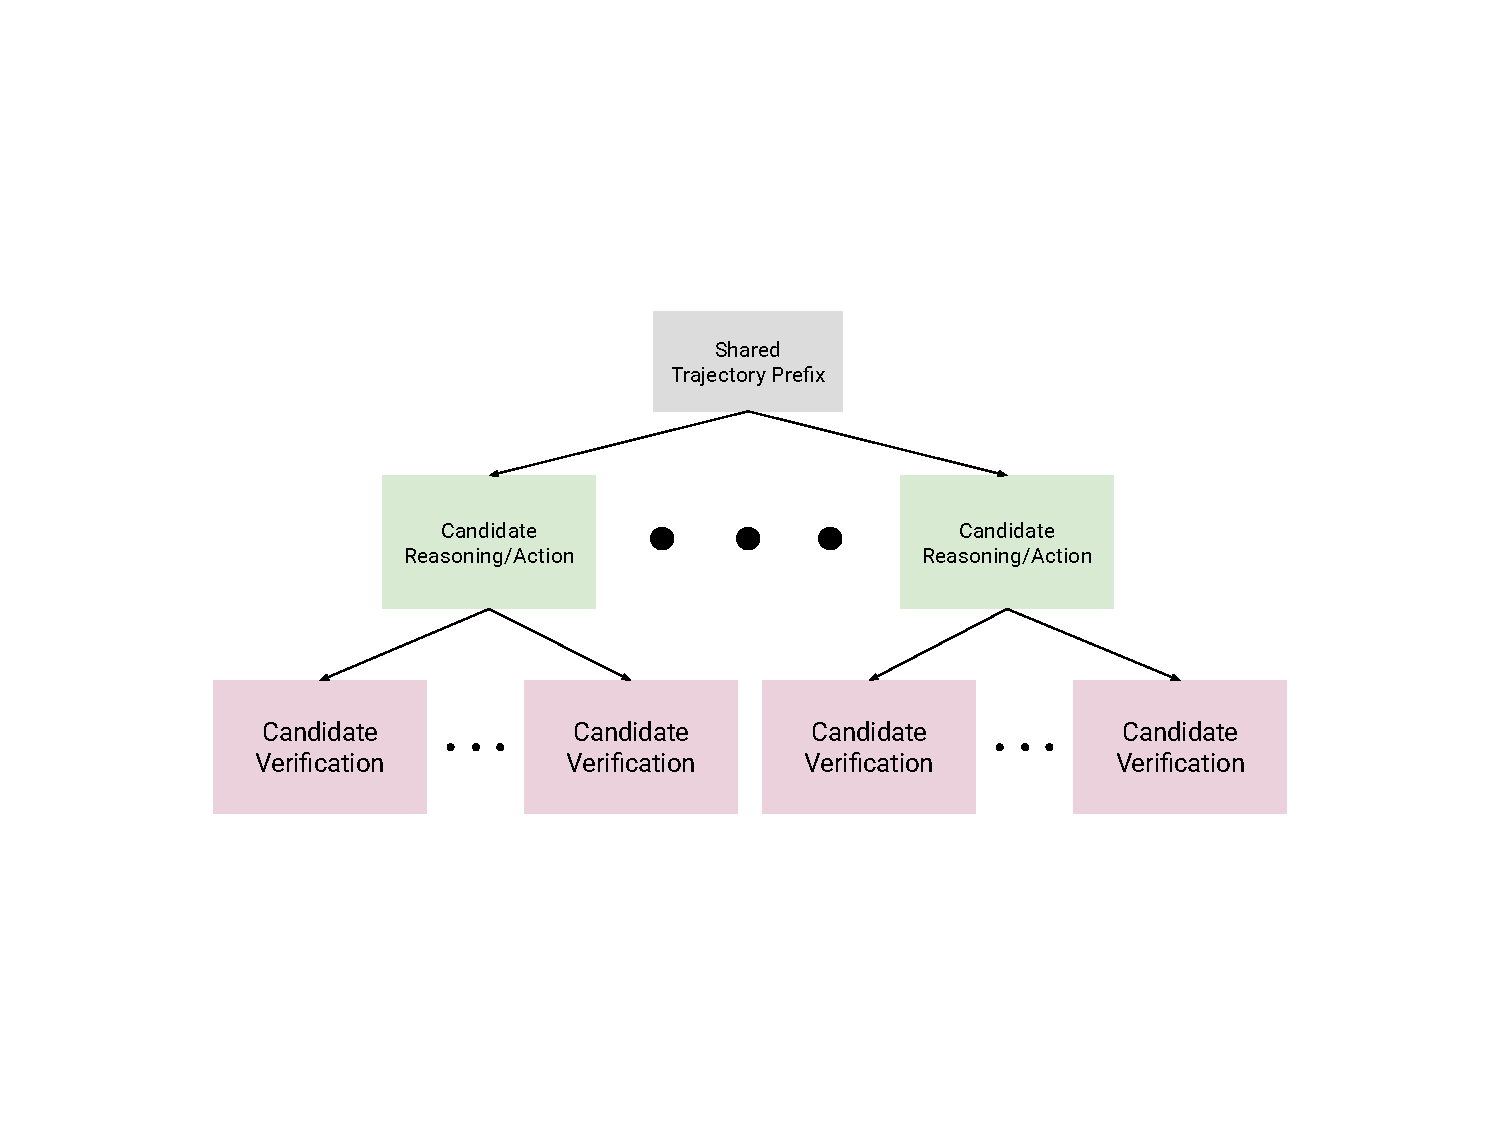
\includegraphics[width=\linewidth]{img/trajectory_gen.pdf}
    \caption{The shared prefix generation tree.}
    \label{fig:shared-prefix}
\end{figure} 

\subsubsection{Initialization, Tool Validation, and Query Construction}\label{sec:init-valid-query}

We define $\text{InitState}(q, e^{\text{user}}, C^{\text{in}})$ as a deterministic function that constructs the initial interpretation $I_0$ and structured state $S_0$ from the query, user-provided evidence, and seed gene set. The working interpretation $I_0$ is populated from a fixed template: the mechanistic claim is empty, the evidence field records only the user-provided inputs, the uncertainty field is blank, and the next subgoal is set to the query $q$. The structured state $S_0$ is initialized as follows:
\begin{enumerate}
    \item the user-provided anchors are set to $(q, e^{\text{user}})$,
    \item the relationship status $rel_0$ is set to \texttt{unknown},
    \item the predicted group is initialized to $G_0 = C^{\text{in}}$,
    \item the evidence log $E_0$ is empty,
    \item the predicted mechanistic labels are empty,
    \item the remaining budget is $T_{\max}$ and the continuation state is $z_0 = \texttt{continue}$.
\end{enumerate}
The agent does not observe the task type $C_{\text{type}}$, the true relationship status, or the hidden target $C$; it must infer the appropriate task case through exploration.

We define $\text{ValidTool}(a_{t,i}, S_t)$ as a deterministic function that checks whether a proposed tool action $a_{t,i}$ is executable given the current structured state $S_t$. Validation proceeds in two stages. First, the syntax check verifies that the tool name referenced in $a_{t,i}$ exists in the current tool vocabulary and that all arguments conform to the tool's input schema. Second, the semantic check verifies that basic conditions are satisfied with respect to the graph environment. For example, the function ensures that queried genes exist in the multiplex, requested layers are valid, and required fields in $S_t$ are populated. If either check fails, $\text{ValidTool}$ returns false and the observation $o_{t,i}$ is set to $\varnothing$. Invalid tool calls are counted toward $n_{inv}$ in the efficiency penalty (Equation~\ref{eqn:eff-pen}).

At inference time, users provide a natural language query $q$ alongside optional evidence $e^{\text{user}}$. Queries are unconstrained and may range from broad exploratory requests to specific hypothesis-driven questions. Evidence may include any combination of:
\begin{enumerate}
    \item a seed gene list,
    \item a multiplex graph or subgraph,
    \item free-text context such as experimental notes or prior findings, and
    \item structured annotations such as GO terms, pathway labels, or expression data from prior analysis.
\end{enumerate}

During training, we simulate this variability by generating diverse queries and evidence configurations from module metadata. For each sampled task $(C^{\text{in}}, C, C_{\text{type}})$, we sample a query from task-type-specific deterministic templates and an evidence mode $\rho \in \{\texttt{minimal}, \texttt{graph}\}$ that controls which evidence types are provided to the agent. Table~\ref{tbl:query-templates} defines representative query templates and compatible evidence modes for each task type. To promote phrasing diversity, we use an LLM to paraphrase each template query into natural language variants conditioned on the gene symbols of the sampled module. All generated queries and evidence configurations are cached during dataset construction for reproducibility.

\begin{table}[ht]
\centering
\caption{Representative query templates and compatible evidence modes by task type. Evidence modes: \texttt{minimal} (seed gene list) or \texttt{graph} (seed gene list + multiplex subgraph).}
\label{tbl:query-templates}
\begin{tabularx}{\textwidth}{l Y l}
\toprule
\textbf{Task type} & \textbf{Example query} & \textbf{Evidence modes} \\
\midrule
\texttt{recovery} & ``What other genes are functionally related to \{seed genes\}?'' & minimal, graph \\
\texttt{refinement} & ``Which of these genes do not belong together?'' & minimal, graph \\
\texttt{explanation} & ``What mechanism connects \{seed genes\}?'' & minimal, graph \\
\texttt{none} & ``Are these genes mechanistically related?'' & minimal, graph \\
\bottomrule
\end{tabularx}
\end{table}

\subsubsection{Branch Ranking, Preference Mining, and Selection}\label{sec:branch-ranking}
Each candidate branch is assigned a deterministic local score computed from the structured state, runtime outputs, and hidden module targets. These local scores are used to rank same-prefix candidates and mine DPO preference pairs against that selection. Because several branches frequently tie or fall within a small margin of each other, continuation selection does not reduce to a strict $\arg\max$, but instead, within a tolerance margin $\epsilon$ of the best normalized score, ties are broken with task-specific heuristics such as prompted seed gene retention and tool-supported evidence, pushing the logged trajectory to favor well-grounded candidates over those that score highly by chance. We defer the formal score definitions to Section~\ref{sec:rewards}.

\subsection{Preference Scoring and Reward Design}\label{sec:rewards}
\subsubsection{Design Principles and Scoreable Objects}
We define all training-time scores over structured state transitions, deterministic runtime metadata, and hidden module-derived targets rather than textual reasoning. This design choice keeps scoring reproducible, machine-parseable, and scalable, while avoiding dependence on human judges or semantic evaluation of natural-language trajectories. We decompose all scores into four components: schema compliance, group membership, mechanistic quality, and efficiency. 

\subsubsection{Deterministic Local Branch Scoring for DPO}
We define local branch scoring for DPO as 

\begin{equation}\label{eqn:local-reward}
    s^{local}_{t,i,j} = w_s\, s^{schema} + w_c\, \Delta s^{module} + w_m\, \Delta s^{mech} - w_e\, p^{eff} - p^{mismatch}
\end{equation}

where $\Delta s^{mech}$ is the evidence-grounded mechanistic quality delta. Additionally, mechanistic quality is clamped to be non-positive when the candidate degrades the predicted group relative to the task type (e.g. by adding noise genes during recovery or removing true members during refinement), and $p^{mismatch}$ penalizes an \texttt{explanation} candidate that reduces recovery of an already-complete module.

We define $s^{schema}_{t,i,j}$ as a binary indicator that equals 1 if the candidate's structured state and interpretation updates are schema valid, and 0 otherwise. Specifically, schema compliance is defined by a properly-formed JSON with all required fields present and tool calls referencing valid tool names and arguments. We formalize this term as
\begin{equation}\label{eqn:schema-score}
   s^{schema}_{t,i,j} = \mathbf{1}(\text{SchemaValid}(c_{t,i,j})).
\end{equation}

We use $\Delta s_{module}$ to measure the change in module membership accuracy from step $t$ to $t+1$. Because the runtime state may contain multiple predicted groups, we first score a state by the best-matched predicted group:

\begin{equation}\label{eqn:module-state-score}
    s^{module}(z; C, C_{\text{type}}) =
    \max_{G \in \mathcal{G}(z)}
    \left[
        \alpha J(G, C) + \beta P(G, C) + \gamma R(G, C)
    \right],
\end{equation}

where $\mathcal{G}(z)$ denotes the set of predicted groups in state $z$, with an empty group used when no prediction is present. We then define the local module improvement as

\begin{equation}\label{eqn:module-score}
        \Delta s^{module}_{t,i,j}
    =
    s^{module}(z_{t+1,i,j}; C, C_{\text{type}})
    -
    s^{module}(z_t; C, C_{\text{type}}).
\end{equation}

where $J$, $P$, and $R$ denote Jaccard, precision, and recall respectively, the weights $\alpha, \beta, \gamma$ are set per task type. Recovery upweights recall ($\alpha,\beta,\gamma = 0.2, 0.2, 0.6$) to reward found members, refinement upweights precision ($0.2, 0.6, 0.2$) to penalize retained noise, and explanation weights them equally ($\tfrac{1}{3}$ each). This best-group formulation supports the multiple-groups state representation while keeping the hidden target single-module for scoring.

We define the mechanism quality of a state as an evidence-grounded score $m_t \in [0,1]$. From the evidence log, we extract three support signals: enrichment support $e_t$, annotation support $g_t$ (from \texttt{query\_mygene}), and network support $u_t$, each $\in [0,1]$. We define a consensus term $\kappa_t = \max(e_t, g_t)$, a cross-tool agreement term $\chi_t = \min(e_t, g_t)$, an evidence strength term $\sigma_t = \max(e_t,\ 0.75\,g_t,\ 0.5\,u_t)$, and an annotation-only strength term $\sigma^{\text{ann}}_t = \max(e_t,\ 0.75\,g_t)$. We additionally compute a grounding term $\gamma_t$ (claim entities are supported by observed evidence), a specificity term $\psi_t$ (vague or generic claims are penalized), a stability term $b_t$ (enrichment consistency across query subsets), and a discounted network-agreement term $\hat{u}_t = u_t$ if $\kappa_t > 0$ and $0.35\,u_t$ otherwise. An abstention term $\alpha_t$ rewards withholding a claim under weak support: $\alpha_t = 1 - \sigma_t$ when the state abstains (relationship status is \texttt{insufficient\_support} or an abstaining claim), $0$ when an unsupported claim is asserted ($\sigma_t \le 0.05$), and $0.5$ otherwise.

The score takes one of two branches depending on whether the state abstains:
\[
    m_t = \begin{cases}
        0.60\,\alpha_t + 0.20\,\hat{u}_t + 0.20\,\gamma_t & \text{(abstaining)} \\[4pt]
        0.25\,\gamma_t + 0.25\,\kappa_t + 0.18\,\psi_t + 0.12\,\hat{u}_t + 0.10\,b_t + 0.10\,\chi_t & \text{(asserting)}
    \end{cases}
\]

In the asserting branch, the score is multiplied by $0.35$ when a claim or labels are present but unsupported ($\sigma_t \le 0.05$). In the abstaining branch $m_t$ is forced to $0$ for any non-\texttt{none} task whose annotation evidence is absent ($\sigma^{\text{ann}}_t \le 0.05$), preventing weak-evidence abstention from being rewarded on tasks that should produce a grounded group. The per-step mechanism reward is the change $\Delta s^{mech}_{t,i,j} = m_{t+1,i,j} - m_{t,i,j}$, set to $0$ if no mechanistic claim has been made.

$p_{eff}$ is a small penalty designed to discourage two behaviors: excessively long trajectories and invalid tool calling. Long trajectories are penalized via the term $t / T_{\max}$, while we count invalid tool calls (those that are schema-invalid, exact duplicates, or return empty observations) with $n_{inv}$, penalizing them proportionally to the total number of tool calls: $(n_{inv} / n_{total})$. We formalize this scoring term as
\begin{equation}\label{eqn:eff-pen}
    p^{eff}_{t,i,j} = \lambda_1 (t / T_{\max}) + \lambda_2(n_{inv} / n_{total}).
\end{equation}

For the \texttt{none} task type, where the hidden target is empty, the membership component is replaced by an abstention score
\[
    s^{none} = w_{rel}\, \mathbf{1}[rel = \texttt{insufficient\_support}] + w_{abs}\, \mathbf{1}[G = \varnothing],
\]

with $w_{rel} = 0.6$ and $w_{abs} = 0.4$. This rewards the agent both for declaring no shared mechanism and for refusing to emit a spurious group.

\subsubsection{Terminal Reward Decomposition for GRPO}\label{sec:terminal-reward}
Unlike DPO, which compares local same-prefix branches, policy gradient methods require a scalar reward for a completed rollout. We therefore define a terminal reward over the final structured state and trajectory log:

\begin{equation}\label{eqn:terminal-reward}
    R_T = w^T_s s^T_{schema} +w^T_{abs} s^{T}_{module} + w^T_{c} \Delta s^{T}_{module} + w^T_{mabs} s^T_{mech} + w^T_{m} \Delta s^{T}_{mech} - w^T_e p^{T}_{eff}. 
\end{equation}

While all terms included in local scoring appear in the terminal reward, they are modified to capture global behavior. Additionally, two new rewards are included to capture absolute recovery. Absolute terms appear in the terminal score but not the local score. Because local scoring is evaluated on examples that share the same starting state $S_t$, absolute levels cancel, and only relative metrics matter. Conversely, the terminal reward is evaluating complete trajectories, which may vary in starting difficulty and length, so absolute metrics capture global problem-solving ability.

We define the absolute module membership score as the composite Jaccard, precision, and recall evaluated on the final predicted group $G_T$ against the hidden target $C$:
\begin{equation}\label{eqn:terminal-module-abs}
    s^{T}_{module} = \alpha J(G_T, C) + \beta P(G_T, C) + \gamma R(G_T, C),
\end{equation}
using the same weighting coefficients $\alpha, \beta, \gamma$ defined in Equation~\ref{eqn:module-score}. The cumulative module delta is the difference between the final and initial composite scores:
\begin{equation}\label{eqn:terminal-module-delta}
    \Delta s^{T}_{module} = s^{T}_{module} - s^{0}_{module},
\end{equation}
where $s^{0}_{module} = \alpha J(G_0, C) + \beta P(G_0, C) + \gamma R(G_0, C)$ is the composite score at initialization.

The absolute mechanism score is the evidence-grounded mechanism quality $m_T$ of the final state:
\begin{equation}\label{eqn:terminal-mech-abs}
    s^{T}_{mech} = m_T.
\end{equation}
The cumulative mechanistic delta is the corresponding difference:
\begin{equation}\label{eqn:terminal-mech-delta}
    \Delta s^{T}_{mech} = m_T - m_0.
\end{equation}
If no mechanistic claim has been made at termination, we set $s^{T}_{mech} = 0$ and $\Delta s^{T}_{mech} = 0$.

The terminal schema score checks that the final structured state is schema-valid and that the termination mode is properly recorded:
\begin{equation}\label{eqn:terminal-schema}
    s^{T}_{schema} = \mathbf{1}(\text{SchemaValid}(S_T) \land \text{TerminationRecorded}(S_T)).
\end{equation}

Finally, the terminal efficiency penalty aggregates trajectory length and invalid tool use across all steps:
\begin{equation}\label{eqn:terminal-eff}
    p^{T}_{eff} = \lambda_1 \left(\frac{T}{T_{\max}}\right) + \lambda_2 \left(\frac{\sum_{t=0}^{T-1} n^{t}_{inv}}{\sum_{t=0}^{T-1} n^{t}_{total}}\right).
\end{equation}

\subsubsection{Preference Pair Construction, Score Normalization, and Filtering}\label{sec:pref-construction}
At each decision point $t$, we create DPO preference tuples of the form $(x_t, c_t^+, c_t^-)$ from our candidate set $\mathcal{C}_t = \{c_{t,i,j}\}$. We define $x_t = (q, e^{\text{user}}, I_t, S_t)$ as the shared-prefix context and $c_{t,i,j}$ as a sample interpretation continuation from Algorithm~\ref{alg:trajectory-gen}. Each continuation contains the model-generated reasoning step, tool action, verifier update, and continuation decision.

Before constructing pairs, we normalize scores to ensure that the selection margin has a consistent meaning across task types and trajectory lengths. We apply min-max normalization within each candidate pool $\mathcal{C}_t$, rescaling the composite local scores to $[0, 1]$. We denote the normalized score of candidate $c_{t,i,j}$ as $\bar{s}^{\,\text{local}}_{t,i,j}$.

To create paired examples, we set the preferred candidate $c_t^+$ to the branch selected as the trajectory continuation, $c_{t,i^\star, j^\star}$ (Section~\ref{sec:branch-ranking}), rather than to a strict $\arg\max$ of the normalized score. Because selection resolves near-ties with task-specific heuristics within a tolerance $\epsilon$, the preferred branch is the one judged best for the task, not merely the highest-scoring candidate. We then define a selection margin $\tau$ and drop all candidates for which

\[
    \bar{s}^{\,\text{local}}_{t,i^\star,j^\star} - \bar{s}^{\,\text{local}}_{t,i,j} < \tau,
\]

where $(i^\star, j^\star)$ indexes the selected candidate. This prevents the construction of pairs that are near ties. The remaining candidates form the eligible dispreferred pool $\mathcal{C}_t^{-}$.

From $\mathcal{C}_t^{-}$, we draw dispreferred examples across three difficulty bins, $d \in \{\texttt{easy}, \texttt{medium}, \texttt{hard}\}$. We construct $\texttt{easy}$ pairs by selecting the lowest-scoring candidate in $\mathcal{C}_t^{-}$, $\texttt{medium}$ pairs by selecting the candidate with the median score, and $\texttt{hard}$ pairs by selecting the highest-scoring candidate in $\mathcal{C}_t^{-}$.

We store each preference pair $(x_t, c_t^+, c_t^-)$ along with its difficulty bin $d$, task type $C_{\text{type}}$, decision step $t$, raw and normalized scores, and the score margin in the preference corpus $\mathcal{P}$. After trajectory generation is complete, we rebalance $\mathcal{P}$ across task types and difficulty bins by downsampling overrepresented categories to ensure that the training distribution is not dominated by task types that produce disproportionately many informative pairs. The curriculum strategy described in Section~\ref{sec:curriculum} controls which difficulty bins are included at each training stage.

\subsubsection{Mechanistic Rendering and Training Outputs}
Each selected trajectory is logged as a sequence of turn records, from which we render short per-step findings and a final mechanistic summary. These artifacts are then converted into SFT trajectory examples, evidence-to-finding records, and DPO preference pairs for the downstream training pipeline. Additionally, scored trajectories can be utilized for policy gradient optimization, such as PPO or GRPO.

\subsection{Training Pipeline}\label{sec:training}
We propose a training pipeline that closely aligns with standard model post-training pipelines. First, we utilize supervised fine-tuning for general biological knowledge and tool calling. We continue training with DPO on stepwise interpretation tree comparisons. Finally, we promote novel exploration over long-horizon tasks with policy gradient optimization.

\subsubsection{Warm-Start SFT}\label{sec:warmstart}
We first train our policy model with warm-start SFT using the closed-book dataset outlined in Section~\ref{sec:data}. We will train our policy model on OLCF's Frontier Supercomputer~\cite{frontier}, utilizing slurm~\cite{slurm} for job scheduling, huggingface and TRL~\cite{trl} for weight updating, DeepSpeed ZeRO-3 for model parallelism~\cite{deepspeed}, Low-Rank Adaptation for parameter-efficient fine-tuning~\cite{hu2022lora}, Weights and Biases~\cite{wandb} for tracking convergence, and gpt-oss-120b~\cite{gpt-oss} as our base policy. We will utilize early stopping checkpointing to prevent model overtraining.

\subsubsection{Tool-Call and Evidence-to-Finding SFT}
We continue the supervised fine-tuning stage by adding open-book tool calling examples and evidence-to-finding examples to our data mixture. We initialize our policy from the warm-start SFT checkpoint with the lowest loss, and we utilize the same pipeline for model training.

\subsubsection{DPO Training}
After training our model via SFT, we will utilize its learned domain knowledge and tool calling capabilities to perform DPO training. We will utilize examples generated with the trajectory construction methods specified in~\ref{sec:shared-prefix} to create paired preference data. Branch continuations will be scored using the functions defined in Section~\ref{sec:pref-construction}. At each decision point, the branch selected as the trajectory continuation serves as the preferred candidate $c_t^+$, while dispreferred candidates $c_t^-$ are drawn from the eligible dispreferred pool across the \texttt{easy}, \texttt{medium}, and \texttt{hard} difficulty bins. Model weights will be optimized using the DPO objective function~\cite{dpo}:

\[
\mathcal{L}_{\text{DPO}}(\pi_\theta; \pi_{\text{ref}}) = -\mathbb{E}_{(x, y_w, y_l) \sim \mathcal{D}} \left[ \log \sigma \left( \beta \log \frac{\pi_\theta(y_w | x)}{\pi_{\text{ref}}(y_w | x)} - \beta \log \frac{\pi_\theta(y_l | x)}{\pi_{\text{ref}}(y_l | x)} \right) \right].
\]

Additionally, during training, we will generate trajectories with new, trained model checkpoints to improve our model's generated preference data. This will allow us to continue making model improvements even after scoring is optimized on our initial dataset.

\subsubsection{Online RL for Long-Horizon Exploration}
After training with DPO, we will implement a final GRPO stage for long-horizon exploration. Unlike DPO, GRPO requires no annotated trajectories; rather, optimization is done by calculating the advantage of an output relative to the rollout group $\{o_1, o_2, \dots, o_G\}$ using the function

\begin{multline*}
    \mathcal{J}_{GRPO} = \mathbb{E}[q \sim P(Q), \{y_i\}_{i=1}^{G} \sim \pi_{\theta_{old}}(Y\mid q)] \\
    \frac{1}{G} \sum_{i=1}^{G}\frac{1}{\mid y_i \mid} \sum_{t=1}^{\mid y_i \mid} \Bigg \{ \text{min} \Big [ \frac{\pi_\theta (y_{i,t}\mid q, y_{i, <t})}{\pi_{\theta_{old}}(y_{i,t}\mid q, y_{i, <t})} \hat A_{i,t}, \text{clip} \Big( \frac{\pi_\theta (y_{i,t}\mid q, y_{i, <t})}{\pi_{\theta_{old}}(y_{i,t}\mid q, y_{i, <t})}, 1 - \varepsilon, 1 + \varepsilon \Big) \hat A_{i,t} \Big] \\
    - \beta \mathbb{D}_{KL} [\pi_\theta \mid\mid \pi_{ref}] \Bigg \},
\end{multline*}

where 

\[
\hat A_{i,t} = \tilde{r}_i  = \frac{R^{T}_i - \text{mean}(R^{T})}{\text{std}(R^{T})}
\]

By foregoing structured, annotated preference pairs, GRPO promotes novel exploration for problem solving. We aim to utilize this policy gradient method to prevent mode collapse in exploration trajectories and reinforce full coverage of the exploration space. The reference policy $\pi_{ref}$ is fixed at the DPO checkpoint that initializes GRPO and is not updated during online rollouts, so the KL term anchors exploration to a stable reference rather than drifting with the trained policy.

\subsection{Curriculum and Optimization Strategy}\label{sec:curriculum}
We will employ a training curriculum throughout the optimization process, scaling problem difficulty with model performance. 

During the SFT stage, we scale difficulty by moving from closed-book biological questions to open-book biological questions that require tool use. This promotes learning biological understanding first, and then moving to structured, schema-respecting tool calling tasks second.

After training a joint closed- and open-book SFT checkpoint, we scale difficulty for DPO pairs by training on increasingly difficult examples, based on difficulty bins defined in Section~\ref{sec:pref-construction}. We begin DPO training by limiting preference pairs to $d = \texttt{easy}$ examples, then adding $\texttt{medium}$ and $\texttt{hard}$ examples as training saturates for each difficulty. After DPO training converges on $\texttt{hard}$ preference pairs, we transition to online RL to promote exploration beyond the behaviors captured in logged trajectory outputs.

We scale long-horizon reinforcement learning difficulty with several strategies. First, we modulate the trajectory length $T_{\max}$, starting with shorter exploration budgets and gradually increasing exploration length for problems that require multi-hop exploration. Additionally, we modulate realized module size, beginning training on small modules and shifting to larger ones as rewards saturate. Finally, we scale the per-task difficulty level, which jointly controls the number of dropped and added genes and the source-specific distractor band from which noise and \texttt{none} genes are drawn: dendrogram-distance bands for \textsc{Mentor}-derived modules (Section~\ref{sec:mentor-corpus}) and post-elbow rank bands for RWR-LOE modules (Section~\ref{sec:loe-corpus}). Higher difficulties remove or add more genes and draw distractors from nearer, more easily confused regions of the corresponding module source, making recovery and refinement harder. At each stage, training batches are sampled from both the \textsc{Mentor}-derived and RWR-LOE module pools and are rebalanced by task type and difficulty bin to prevent either corpus from dominating training.

\subsection{Evaluation and Benchmarks}\label{sec:eval}
\subsubsection{Module Holdout Evaluation}
We will use several metrics to evaluate the effectiveness of our model. Each metric will be calculated by parsing the model's terminal structured state $S_T$, allowing for scalable evaluation of our checkpoints. All evaluations will be conducted on a held out set of \textsc{Mentor}- and RWR-LOE-derived modules from the brain multiplex.

We will report four metrics for evaluation: Jaccard index $J$, precision $P$, recall $R$, and $F_1$ score on the predicted module $C^{pred}$ vs. the hidden module target $C$. Jaccard index is defined as 
\[
    J(C^{pred}, C) = \frac{\mid C^{pred} \cap C \mid}{\mid C^{pred} \cup C \mid},
\]
penalizing both missing and extra entities. Precision is defined as
\[
    P = \frac{TP}{TP + FP},
\]
measuring the proportion of true positive entities compared to all predicted positives. Recall is defined as
\[
    R = \frac{TP}{TP + FN},
\]
measuring the proportion of true positive predictions to the sum of true positives and false negatives. The F1 score is defined as the harmonic mean of precision and recall,
\[
    F1 = \frac{2}{\frac{1}{P} + \frac{1}{R}},
\]
providing a balanced view of precision and recall to measure general performance. In addition to these module recovery metrics, we will measure mechanistic grounding quality, defined in Equation~\ref{eqn:terminal-mech-abs}, to assess whether mechanistic claims are supported by retrieved evidence.  

We will report the weighted composite reward $R_T$, defined in Section~\ref{sec:terminal-reward}, to directly compare training reward magnitude on validation and holdout splits. If the task type is \texttt{none}, meaning $C = \varnothing$, we will parse the $S_T$ for the predicted relationship $rel_T$. Along with computing global accuracy, we will distinguish between both error directions, analyzing when the model claims no mechanism exists for truly related gene sets and when the model fabricates a mechanism for truly unrelated entities.

Furthermore, we will report efficiency metrics, such as mean trajectory length, budget utilization, and invalid tool call rate. This allows for comparison between holdout efficiency and validation efficiency metrics computed in Equation~\ref{eqn:terminal-eff}.

In addition to general evaluation, we will stratify our evaluation across several axes: module size, noise, task type, and module source. We will divide module size and noise into three discrete bins each for comparative evaluation. Reporting stratified metrics allows us to analyze how \textsc{Mentor-RL} performs as task difficulty increases and task type changes, and comparing metrics by module source exposes whether the model generalizes across module construction methods or exhibits biases toward one of the two module types.

\subsubsection{Novel-Domain Evaluation}
Because the holdout split above is drawn from the same brain multiplex used for training, it measures in-distribution generalization. To assess out-of-distribution performance, we additionally evaluate on \textsc{Mentor}-derived modules from independently published multiplex studies the model was not trained on, such as networks built for opioid use disorder and cardiac studies. These modules are produced by the same \textsc{Mentor} dendrogram procedure (Section~\ref{sec:mentor-corpus}) over different tissue- and disease-specific multiplexes, so they share the module-recovery scoring methodology while presenting genuinely novel network context. We report the same metrics defined in Section~\ref{sec:eval} and expect a performance gap relative to the brain-multiplex holdout, reflecting distribution shift. Because these modules derive from real experimental networks with expert- and algorithm-verified structure, they let us characterize the strengths and limitations of \textsc{Mentor-RL} on real-world, out-of-distribution data.

\subsubsection{Blind Comparative Evaluation}\label{sec:blind-eval}
In conjunction with empirical validation, which measures model accuracy, we will conduct blind comparative evaluations to measure expert domain scientists' model preferences. First, we will perform an inter-model preference test, supplying interpretation outputs from \textsc{Mentor-RL}, GPT-5~\cite{gpt5}, gpt-oss-120b~\cite{gpt-oss}, LLaMA 4~\cite{llama4}, Kimi K2~\cite{kimik2}, and Nemotron 3 Super~\cite{nemotron3}. We will provide between 5 and 15 domain experts with paired samples containing \textsc{Mentor-RL} outputs and outputs from another randomly selected model. We will then ask scientists to indicate their preferred interpretation, and with this information, we will calculate the proportion of \textsc{Mentor-RL} outputs that are preferred compared to other models. To support interpretation of these proportions, we will overlap a subset of evaluation pairs across raters and report inter-expert rating reliability.

After conducting inter-model preference testing, we will perform intra-model preference testing to compare preferences for different model checkpoints. Using the same protocol described for inter-model comparative evaluation, we will compare the base, SFT, DPO, and GRPO-trained \textsc{Mentor-RL} checkpoints. Blind comparative testing will allow us to evaluate model characteristics such as style, tone, and concision that are not easily evaluable with empirical metrics.

\subsubsection{Efficiency and Ablations}
To ensure that each component of our methodology contributes to an improvement in mechanistic interpretation, we will ablate both training stages and design elements. All ablations will be evaluated using the holdout metrics defined in Section~\ref{sec:eval}.

We will ablate phases of our training pipeline to confirm that each stage improves over the previous checkpoints. First, we will test our SFT-only checkpoint compared to the SFT- and DPO-trained checkpoint to ensure that preference optimization yields interpretation gains. Next, we will compare the DPO checkpoint to the full training pipeline to determine whether long-horizon RL training leads to improvement over local preference training. Finally, we will examine the effects of training with only closed-book SFT data vs. a mixed closed- and open-book training set to evaluate whether tool-calling examples in SFT lead to better DPO optimization.

Along with testing various training stages, we will ablate architectural and reward decisions. First, we will ablate the policy's verifier mode, removing it to test whether self-verification is useful for producing better results. Additionally, we will remove the efficiency penalty $p^{eff}$ from the reward to test whether \textsc{Mentor-RL} can learn reasonable trajectory lengths without regularization. Finally, we will ablate difficulty bins in our training curriculum, training on all difficulty bins simultaneously rather than staging them progressively. This ablation will allow us to examine whether the model can learn from hard examples without curriculum staging.

\section{Expected Results and Deliverables}

\subsection{Expected Empirical Results}
We expect \textsc{Mentor-RL} to recover held-out \textsc{Mentor}-derived and RWR-LOE modules with a composite $F_1$ competitive with frontier models at substantially lower per-query inference cost while improving monotonically across the training pipeline. Each of the SFT, DPO, and GRPO checkpoints should outperform the preceding one on module recovery and mechanistic grounding. Under the stratified evaluation defined in Section~\ref{sec:eval}, we expect the largest gains on \texttt{recovery} and \texttt{refinement} tasks, where deterministic graph operators provide dense supervisory signals, and smaller but nontrivial gains on \texttt{explanation} and \texttt{none} tasks, where reward is driven by mechanistic grounding and abstention rather than set-level recovery. On the novel-domain evaluation against experimentally-derived \textsc{Mentor} modules, we expect a performance gap relative to brain multiplex holdout, reflecting distributional shift, but with the gap narrowing as curriculum difficulty and noise levels increase during training. We expect comparable $F_1$ on held-out RWR-LOE modules relative to \textsc{Mentor}-derived modules given the shared task structure, with any gap reflecting differences in module coherence between the two construction methods.

\subsection{Expected Behavioral Results}
Beyond empirical accuracy, we expect three behavioral outcomes. First, the act-verify loop should reduce schema-invalid tool calls and unsupported mechanistic claims relative to a verifier-ablated baseline, measured by invalid tool call rate and ungrounded-claim rate on the holdout split. Second, the efficiency penalty should produce shorter average trajectories without loss of recovery accuracy relative to a penalty-ablated baseline. Third, blind comparative evaluation should show that expert scientists prefer \textsc{Mentor-RL} outputs to base-policy outputs at a significantly higher rate, and preferences relative to frontier models should improve across successive training stages.

\subsection{Deliverables}
We will release, under licenses compatible with the underlying data sources, the following artifacts:
\begin{enumerate}
    \item the module-grounded training environment, including the \texttt{ctypes} multiplex runtime, tool vocabulary, and deterministic scoring functions,
    \item train, validation, and test split indices at the module level, together with the code required to reconstruct the raw training corpus and cached API responses,
    \item trained \textsc{Mentor-RL} checkpoints for each stage of the pipeline (warm-start SFT, joint closed- and open-book SFT, DPO, and GRPO),
    \item the evaluation harness, including \textsc{Mentor} module holdout benchmarks, out-of-distribution published multiplex benchmarks, and blind comparative evaluation protocols, and
    \item training and generation code, curriculum configurations, and logged trajectories to support reproducible re-training and ablation.
\end{enumerate}

\subsection{Broader Impact}
By releasing a deterministically-scored, open-source mechanistic exploration agent together with its training environment, we aim to lower the cost of biological interpretation research and establish a reproducible benchmark that does not require proprietary model access. The module-grounded scoring framework is domain-specific, but the underlying pattern, deterministic structured-state rewards over a tool-using policy, is transferable to other scientific settings with curated ground truth.

\section{Discussion and Conclusion}

\subsection{Reproducibility Without Proprietary Judges}
The training pipeline for \textsc{Mentor-RL} foregoes the use of proprietary judge models to ensure reproducibility and compliance with terms of use. Rewards are computed deterministically over structured state transitions and module-derived ground truth (\textsc{Mentor}-derived and RWR-LOE) rather than by semantic evaluation from a frontier model. Trajectories are generated either by sampling the policy under training or by deterministic templating, not by proxy labeling through a closed API. One exception is query paraphrasing during dataset construction, for which we will use an open-source model with a pinned version so that the paraphrasing step can be reproduced without API access. Despite avoiding proprietary models during training, we will still compare \textsc{Mentor-RL} to them through blind comparative evaluation, detailed in Section~\ref{sec:blind-eval}.

\subsection{Limitations}\label{sec:limitations}
Several limitations constrain the scope of the claims we can make with this work.

\textit{Reward-hacking risk.} The composite module-membership score rewards moves toward the hidden target $C$. Since $C$ is never observed directly, the agent cannot short-circuit it, but shortcut policies are still possible. For example, a policy that always returns a single-pass random-walk-with-restart expansion from the seed set will recover a substantial fraction of \textsc{Mentor} modules without genuine multi-step reasoning. The efficiency penalty does not counteract this behavior. We will monitor tool-use entropy and trajectory diversity during training and, if shortcut behavior emerges, introduce adversarially constructed modules or a diversity bonus as mitigations.

\textit{Shared-weight verifier.} The actor and verifier are two prompting modes of the same policy, so DPO and RL updates on one mode also update the other. This introduces a risk of verifier collapse, in which the verifier learns to endorse the actor's proposals regardless of quality. We will monitor the verifier disagreement rate and, if collapse is observed, consider separate LoRA adapters per mode or a consistency regularizer between modes.

\textit{Task difficulty imbalance.} The four task types are constructed uniformly during corpus construction, but they are not of equal difficulty; \texttt{explanation} tasks require no graph modification, while \texttt{refinement} tasks require the verifier to remove members without a tool that directly marks membership. We treat the per-task sampling weights as a hyperparameter and expect to tune them during pilot training.

\textit{Split-level leakage.} Dendrogram modules share genes across different cuts of the tree; therefore, a module-level split does not by itself prevent leakage through genes shared across overlapping modules. We will report overlap statistics between train and held-out splits and, if overlap is material, adopt a gene-overlap-aware split strategy.

\textit{Expert evaluation scope.} The blind comparative evaluation relies on 5 to 15 domain experts making pairwise preference judgments. This sample size supports descriptive comparison but not tight confidence intervals on preference rates, and expert rating reliability will be reported alongside preference proportions.

\subsection{Conclusion}
We have presented \textsc{Mentor-RL}, a proposed open-source reasoning agent for biological mechanistic interpretation, trained through a staged pipeline of supervised fine-tuning, direct preference optimization over shared-prefix trajectory branches, and policy gradient optimization for long-horizon exploration. The training environment grounds rewards in deterministic graph operators and module targets drawn from the \textsc{Mentor}-derived and RWR-LOE corpora, removing proprietary judges from the loop and exposing every optimization signal as a reproducible, structured quantity. We view \textsc{Mentor-RL} as one instance of a broader methodological pattern: domain-specialized scientific agents whose behavior is shaped by deterministic structured-state rewards over curated ground truth, rather than by semantic evaluation from frontier models. If successful, this pattern offers a route toward scientific AI systems that are cheap to deploy, auditable in their reasoning, and reproducible across research groups without centralized model access.

\printbibliography
\end{document}
